\section{Exploratory Data Analysis}\label{Sec:Exploratory}

The exploratory data analysis will be divided in two parts: firstly, summary statistics are calculated for both numeric and categorical variables; secondly, density plots are produced for numerical variables and bar plots for categorical variables. Correlation will also be calculated, but only with respect to price. This subject will be dealt with in subsection \ref{corr}.

\subsection{Descriptive statistics}\label{subsec:descriptive}

Descriptive statistics make the interpretation of the data easier by giving grouping it and thus providing a shorter representation of it \citep{descrstat:2014}.

As in \cite{descrstat:2014} explained there are the general types of descriptive statistics:
\begin{itemize}
\item Measures of central tendency
\item Measures of spread
\item Graphical displays
\end{itemize}

This subsection will focus on the first two, while subsection 
\ref{distrplots} will deal with the third.

Most of these statistics are usually applied to continuous data and even to numerical discrete data.
For this type of data the following statistics of central tendency were calculated:
\begin{itemize}

\item $mean = \frac{1}{N}\sum\limits_{i=1}^{N}x_i$

\item 

\end{itemize}

The median is also the 2nd quantile.

As for spread, we can derive the range from the minimum and maximum $range = max - min$ and we calculate the 1st and 3nd quantile (the 2nd ist just the median) and their difference $IQR = 3Q - 1Q$. They correspond to the 25\% and 75\% of the values. Finally we also derive the standard deviation, which is the squared root of the variance $variance = ......$ (FORMULA OF VARIANCE)


CANNOT LOAD THE RIGHT CODE :(
\lstinputlisting[language=R, firstline=1, escapechar=|, caption={|\textbf{\href{https://github.com/silvia-ventoruzzo/SPL-WISE-2018/blob/master/Helpers/summary_stat_num.R}{summary\_stat\_num.R}}|}]{../Helpers/getmode.R}

With this code one can calculate the descriptive statistics for one variable on the basis of all the data or, if both \textit{constraint\_var} and \textit{constraint\_var} are set, on the basis of some constraint on the data.

This function will then be applied to all the numerical variables to give a result such as in table\ref{table:sumstatnum}.

\begin{table}[H]
\centering
\begin{tabular}{lrrrrrrrr}
  \hline \hline
variable & min & 1Q & median & 3Q & max & iqr & mean & sd \\ 
  \hline
price & 0.00 & 30.00 & 45.00 & 70.00 & 9000.00 & 40.00 & 67.14 & 220.28 \\ 
   \hline \hline
\end{tabular}
\caption{Sample of descriptive table for numeric variables}
\label{table:sumstatnum}
\end{table}

For categorical variables the explained statistics do not work, therefore frequencies and proportions of each factor were calculated.

CANNOT LOAD THE RIGHT CODE :(
\lstinputlisting[language=R, firstline=1, escapechar=|, caption={|\textbf{\href{https://github.com/silvia-ventoruzzo/SPL-WISE-2018/blob/master/Helpers/summary_stat_fact.R}{summary\_stat\_fact.R}}|}]{../Helpers/getmode.R}


\subsection{Distribution plots}\label{subsec:distrplots}

Also for the distribution plots we distinguish between numerical and categorical variables. In the first case a frequency plot has been produced, where also mean, median, 1st and 3rd quantiles are visible.
Unfortunately, many variables present outliers, which were in some cases excluded from the plots for better visualization.

\begin{figure}[H]
\centering
\subfloat[Complete]{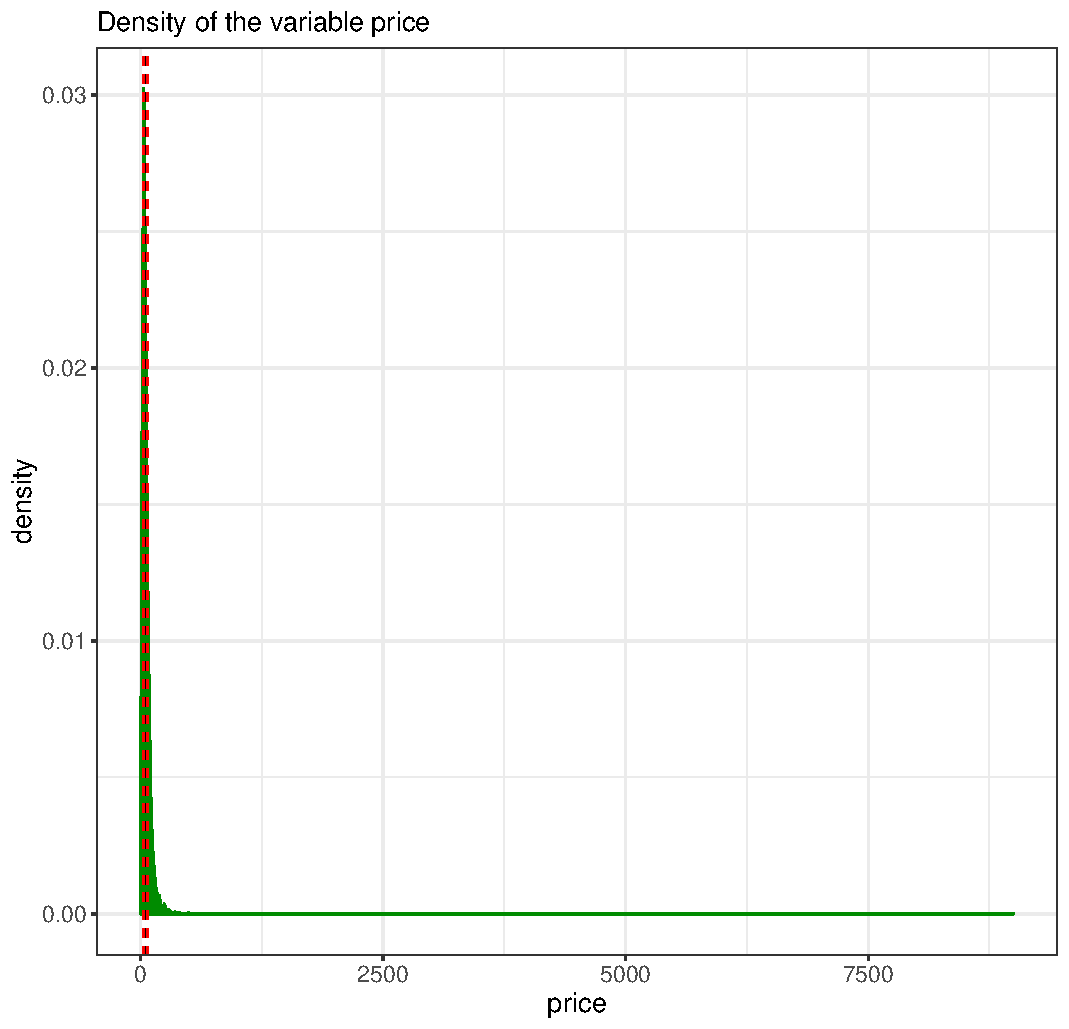
\includegraphics[height=7cm]{price_distribution_complete.pdf}}
\subfloat[Without outliers]{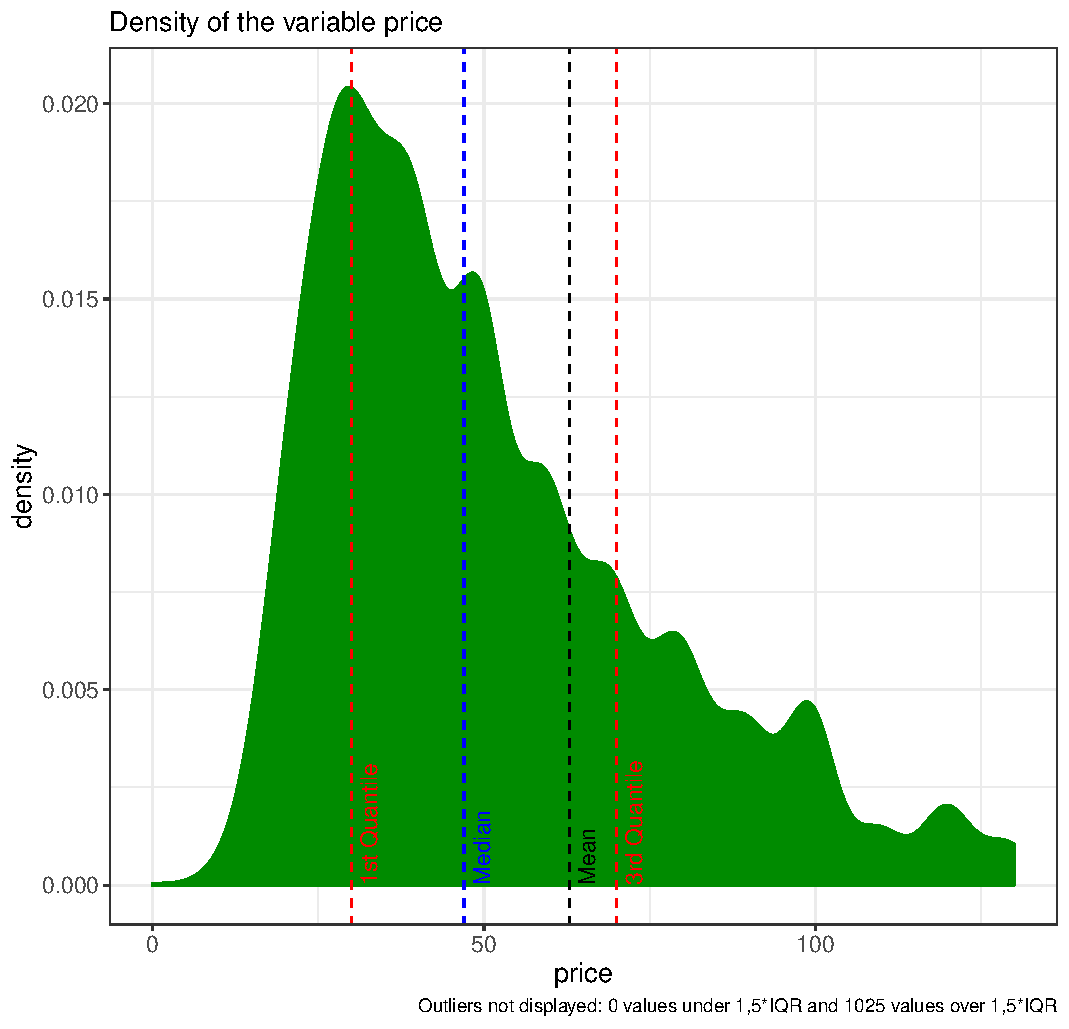
\includegraphics[height=7cm]{price_distribution_nooutliers.pdf}}
\caption{Distribution of the variable price \protect
\includegraphics[scale=0.05]{qletlogo.pdf} {\href{https://github.com/silvia-ventoruzzo/SPL-WISE-2018/blob/master/exploratory_data_analysis.R}{exploratory\_data\_analysis.R}}}
\centering
\end{figure}

For the categorical variables a bar plot is more appropriate, since the values that the variable can assume are discrete and usually also few, like in the case displayed in figure \ref{figure:room_type}.




\begin{figure}[H]
\begin{center}
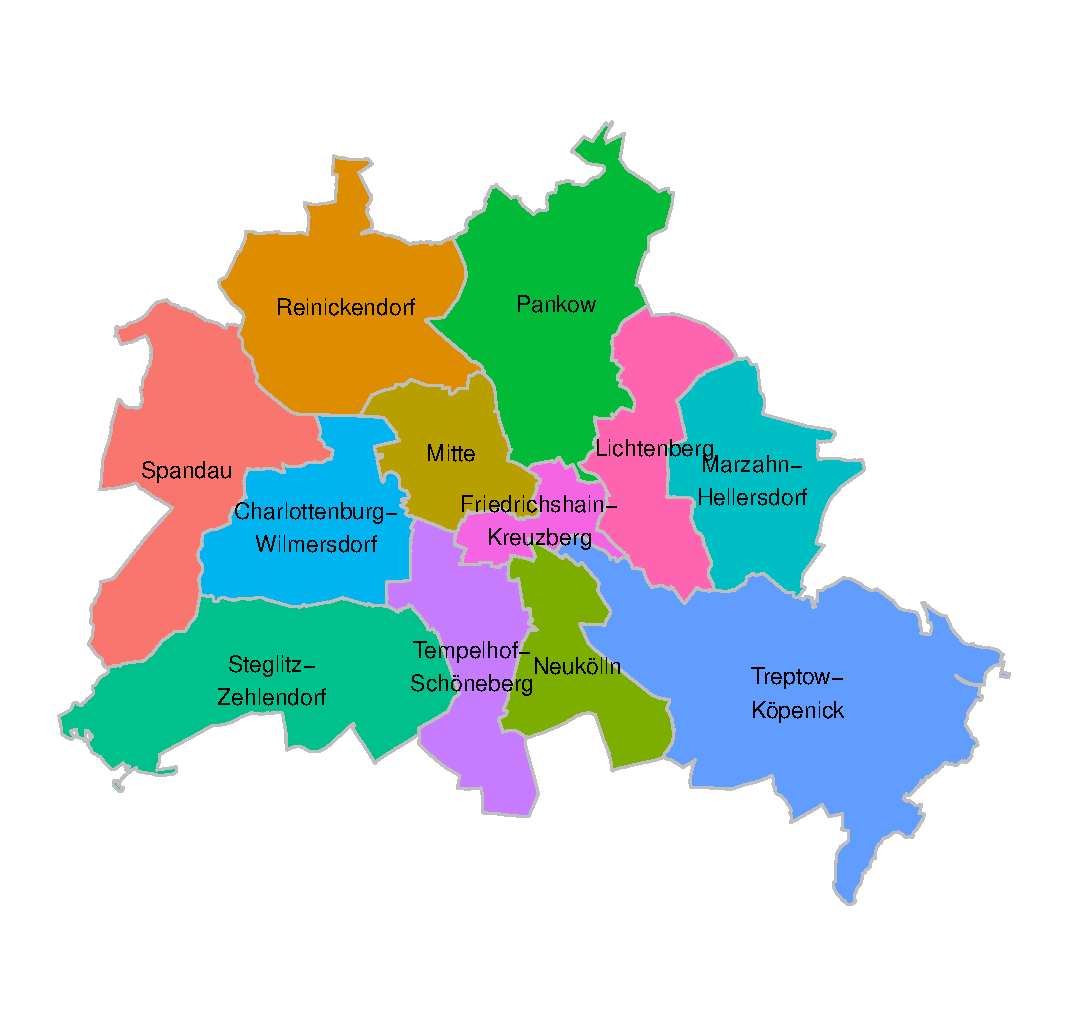
\includegraphics[width=0.5\textwidth, keepaspectratio]{room_type_distribution.pdf} \\
\caption{Distribution of the variable room\_type \protect
\includegraphics[scale=0.05]{qletlogo.pdf} {\href{https://github.com/silvia-ventoruzzo/SPL-WISE-2018/blob/master/exploratory_data_analysis.R}{exploratory\_data\_analysis.R}}}
\label{figure:room_type}
\end{center}
\end{figure}

We also mapped the Berlin districts and the distribution of the average of a certain variable on them with the use of the package \textit{leaflet}.

\begin{figure}[H]
\begin{center}
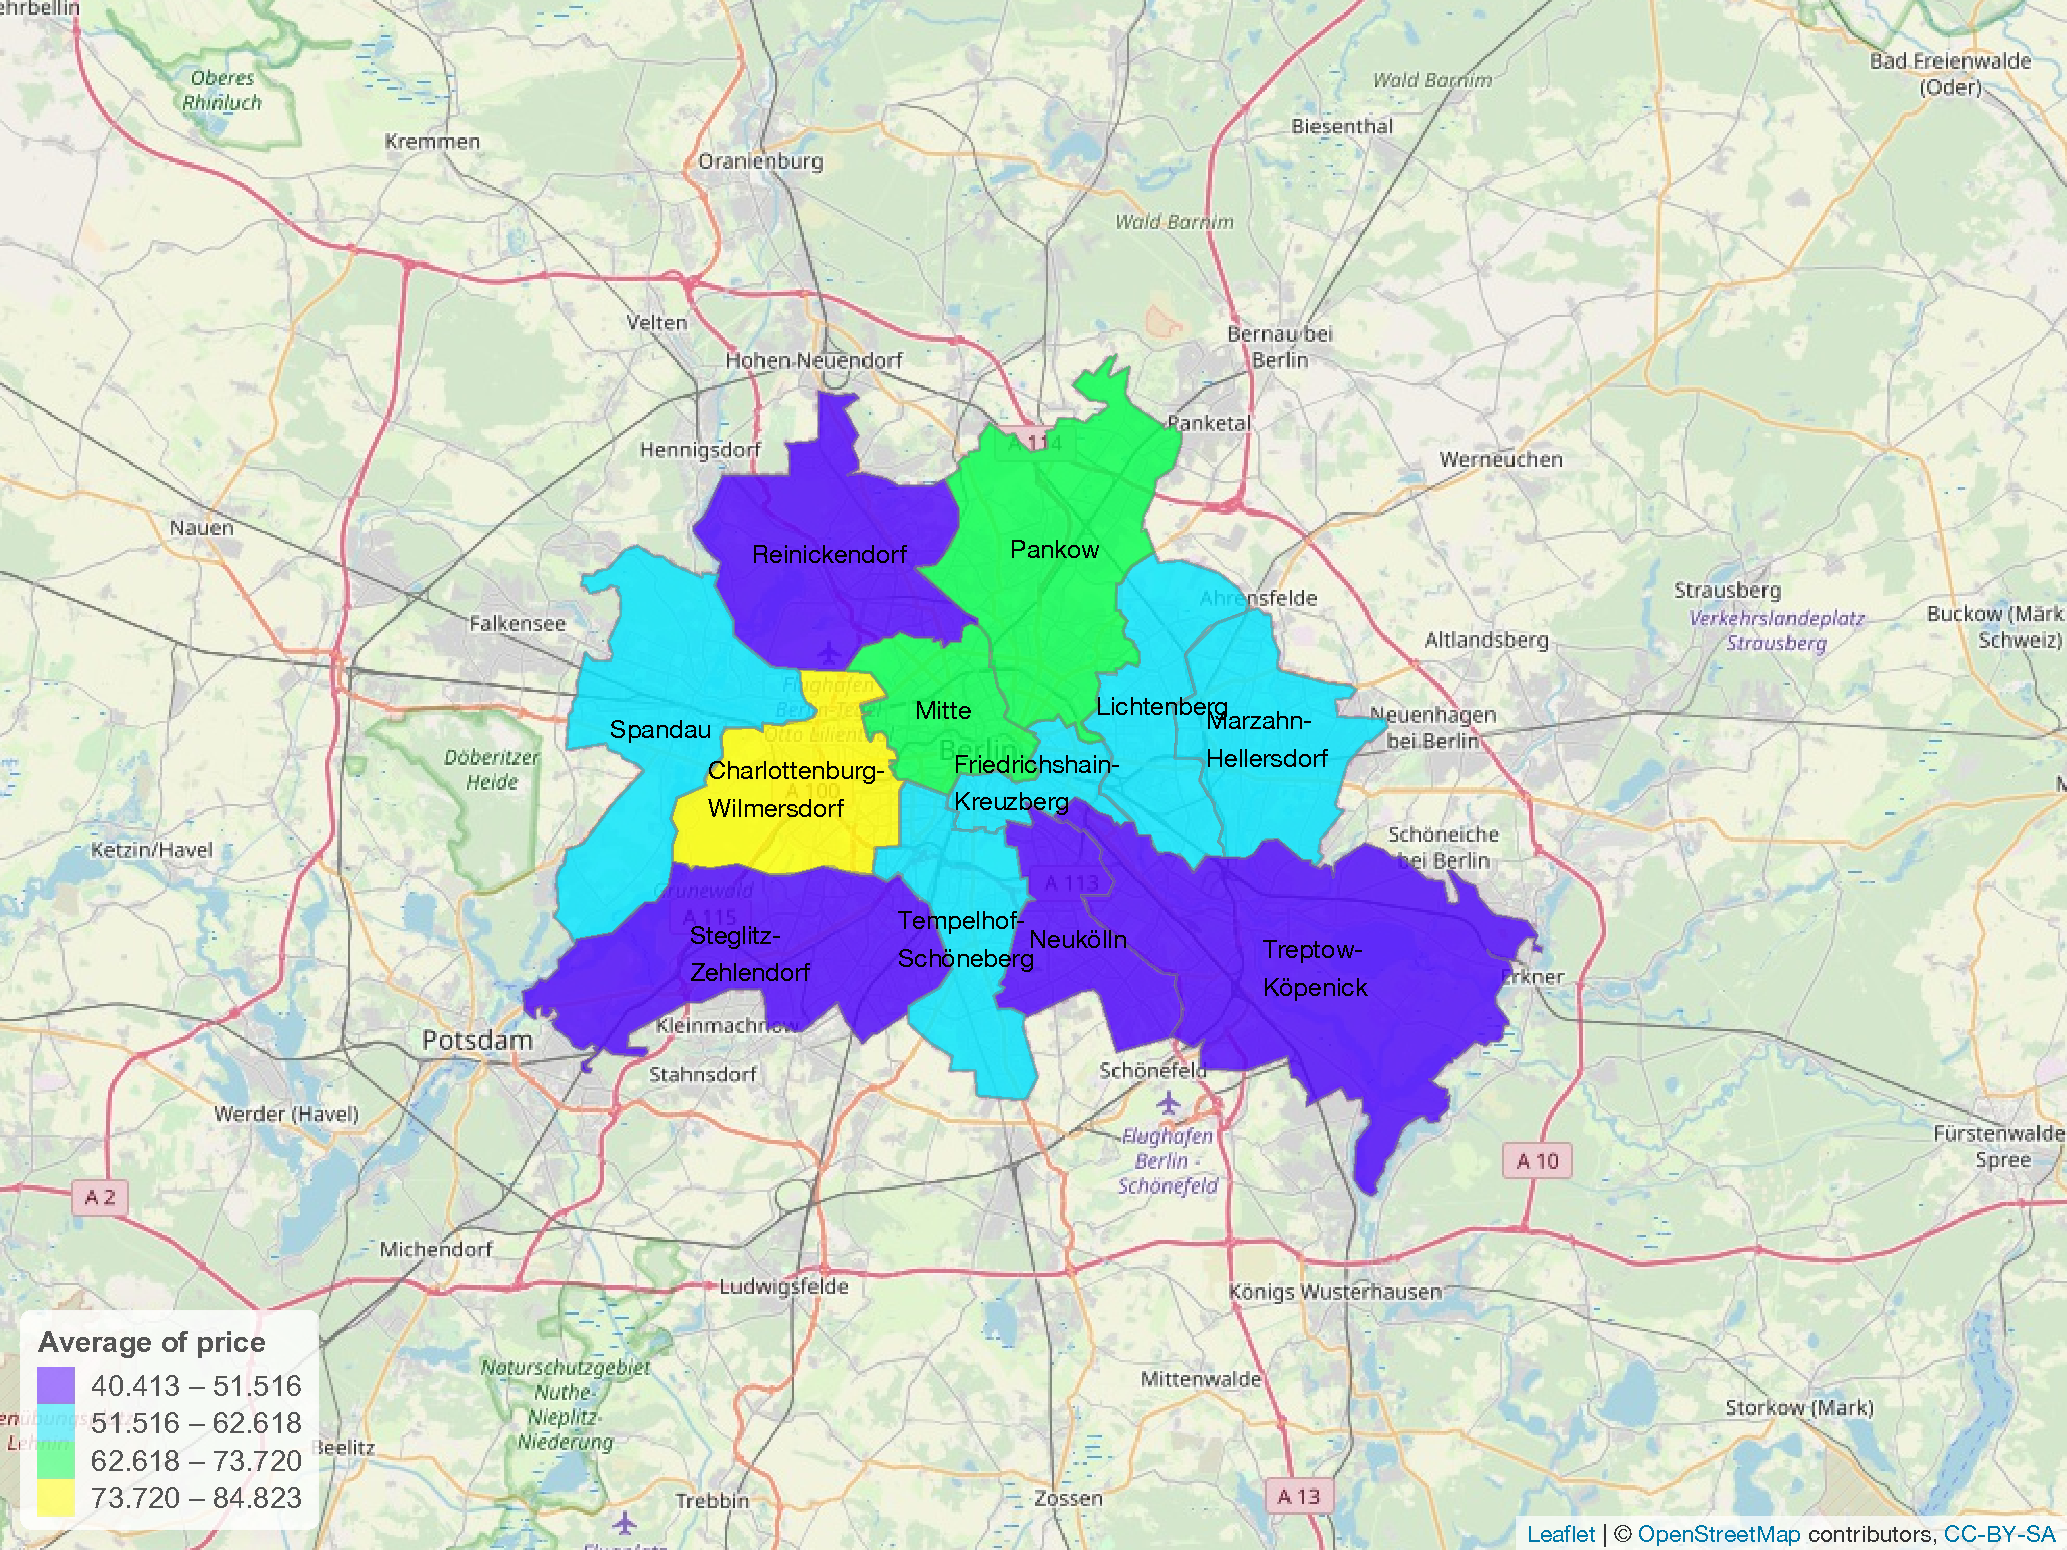
\includegraphics[width=0.5\textwidth, keepaspectratio]{price_map_distr} \\
\caption{Distribution of the average of price across Berlin's districts}
\label{figure:room_type}
\end{center}
\end{figure}